\chapter{Layouts \& Visual Design}
\section{Aims}
\paragraph{} At the end of the practical portion of this topic you will be able to:

\begin{itemize}
\item Use layouts to manage the visual organisation of your views
%\item Fragments
%\item Dialogs (using Fragments)
%\item Action Bar
%\item Orientation
\item Design an app using simple graphical tools
\end{itemize}


\begin{framed}
{\bf{NOTICE:}} In this lab we will be dealing a lot with Views, i.e. user interface elements. In Android Studio you have the option of using the graphical layout tool or editing the layout XML files directly. If you use the graphical tool then it might add extra stuff to your layout file as it attempts to ``help'' you. This is OK but might make things display a little peculiarly. You can always remove these extrabits by editing the XML directly within the file. Either way you should be checking what the graphical editor adds to the XML file so that you become familiar with the underlying source code.
\end{framed}

\begin{framed}
{\bf{NOTICE 2:}} Try to avoid copying and pasting code from the practical notes into your editor. You will learn less this way than you do by typing it in yourself. Typing in the code counts as practise. And practising {\bf{always}} makes you better at the thing you are doing.

Copying and pasting has some additional drawbacks: it might introduce subtle errors into your code from copied white space, you will lose formatting so it is harder to comprehend your code, and you will lose the use of the auto-complete feature which sometimes adds in code, such as import statements.
\end{framed}

\section{Android Layouts}
\paragraph{} A layout is a class that manages the way that child views appear on screen. Anything that is a view or inherits from the View class can be a child of a layout. Layouts also inherit from View so they can be nested within each other. We should take note that there are `layout files', the xml files that you find in the res/layout/ folder, e.g.

\begin{framed}
res/layout/activity\_main.xml
\end{framed}

\paragraph{} and there are also Layout Views, graphical elements that you can use within layout files to organise the user interface elements. In this practical we will be using both aspects of layouts. We will be editing layout files and adding Layout Views to them, as well as other kinds of view. However, we will not spend a lot of time building fully working apps. The aim of this part of the practical is to get a solid understanding of how the different Layouts affect the arrangement of views on screen, but we won't necessarily link the views up to Java code that does things with them That is left as an exercise for you, for example, when a button is displayed, cause it to write out a log line in logcat, or display a Toast, just so that you can get some more practise.

\paragraph{} Android includes a number of standard layouts:

\begin{itemize}
\item Frame Layout
\item Linear Layout (in Horizontal \& Vertical flavours)
\item Table Layout
\item Grid Layout
\item Relative Layout
\end{itemize}

\paragraph{} In this practical we will look at a selection of useful Layouts. So, let's get started.

\paragraph{} Create a new Android project and open the activity\_main.xml layout so that you can edit it. Delete the existing ``Hello World'' text view (by clicking on it and pressing backspace. Now add three buttons to the default RelativeLayout. You should end up with something similar to the following:

\begin{lstlisting}
<RelativeLayout xmlns:android="http://schemas.android.com/apk/res/android"
    xmlns:tools="http://schemas.android.com/tools" android:layout_width="match_parent"
    android:layout_height="match_parent" android:paddingLeft="@dimen/activity_horizontal_margin"
    android:paddingRight="@dimen/activity_horizontal_margin"
    android:paddingTop="@dimen/activity_vertical_margin"
    android:paddingBottom="@dimen/activity_vertical_margin" tools:context=".MainActivity">

    <Button
        android:layout_width="wrap_content"
        android:layout_height="wrap_content"
        android:text="New Button"
        android:id="@+id/button"
        android:layout_gravity="center_vertical" />

    <Button
        android:layout_width="wrap_content"
        android:layout_height="wrap_content"
        android:text="New Button"
        android:id="@+id/button2"
        android:layout_gravity="center_vertical" />

    <Button
        android:layout_width="wrap_content"
        android:layout_height="wrap_content"
        android:text="New Button"
        android:id="@+id/button3"
        android:layout_gravity="center_vertical" />

</RelativeLayout>
\end{lstlisting}
\paragraph{} That's not ideal is it? All the buttons are placed directly on top of each other. We could give each button a specific position, but this would need to be adjusted for different screen sizes, dimensions, and orientations. It is much better to get the Android framework to manage the layout for us (unless we have something extra special that we want to do that the Android layouts can't manage). So let's try out some Layouts....

\subsection{Linear Layout}
\paragraph{} Delete the three buttons from your activity\_main.xml. Add a Horizontal Linear Layout View to your layout file. You should end up with something like this:

\begin{lstlisting}
<RelativeLayout xmlns:android="http://schemas.android.com/apk/res/android"
    xmlns:tools="http://schemas.android.com/tools" android:layout_width="match_parent"
    android:layout_height="match_parent" android:paddingLeft="@dimen/activity_horizontal_margin"
    android:paddingRight="@dimen/activity_horizontal_margin"
    android:paddingTop="@dimen/activity_vertical_margin"
    android:paddingBottom="@dimen/activity_vertical_margin" tools:context=".MainActivity">


    <LinearLayout
        android:orientation="horizontal"
        android:layout_width="fill_parent"
        android:layout_height="fill_parent">
        
    </LinearLayout>
</RelativeLayout>
\end{lstlisting}
\paragraph{} If we run this then we won't actually see very much output as the Layout itself doesn't have any visible view components of its own to display on screen. So we need to add some children to it. Lets put those buttons back but this time as children of the LinearLayout. You should have something like the following:

\begin{lstlisting}
<RelativeLayout xmlns:android="http://schemas.android.com/apk/res/android"
    xmlns:tools="http://schemas.android.com/tools" android:layout_width="match_parent"
    android:layout_height="match_parent" android:paddingLeft="@dimen/activity_horizontal_margin"
    android:paddingRight="@dimen/activity_horizontal_margin"
    android:paddingTop="@dimen/activity_vertical_margin"
    android:paddingBottom="@dimen/activity_vertical_margin" tools:context=".MainActivity">

    <LinearLayout
        android:orientation="horizontal"
        android:layout_width="fill_parent"
        android:layout_height="fill_parent">


        <Button
            android:layout_width="wrap_content"
            android:layout_height="wrap_content"
            android:text="New Button"
            android:id="@+id/button"
            android:layout_gravity="center_vertical" />

        <Button
            android:layout_width="wrap_content"
            android:layout_height="wrap_content"
            android:text="New Button"
            android:id="@+id/button2"
            android:layout_gravity="center_vertical" />

        <Button
            android:layout_width="wrap_content"
            android:layout_height="wrap_content"
            android:text="New Button"
            android:id="@+id/button3"
            android:layout_gravity="center_vertical" />

    </LinearLayout>
</RelativeLayout>

\end{lstlisting}

\paragraph{} Now when you run your app you should see the buttons arranged in a horizontal line across the middle of your screen.

\paragraph{} Now change the orientation parameter of your LinearLayout to vertical so we can try out another orientation of the buttons. 

\begin{lstlisting}
        android:orientation="vertical"
\end{lstlisting}

\paragraph{} When you run the app now you should see that the arrangement of the buttons is in a vertical line but that they are in the top left corner. Let's neaten that up a little by adding a gravity parameter to out LinearLayout:

\begin{lstlisting}
        android:gravity="center"
\end{lstlisting}

\paragraph{} Your vertical buttons should now be centered nicely on screen.

\subsection{Table Layout}
\paragraph{} This is similar to working with a spreadsheet or HTML table. This layout uses TableRow views to organise your views. Create a new project and add a TableLayout to your activity\_main.xml so that you have the following:

\begin{lstlisting}
<RelativeLayout xmlns:android="http://schemas.android.com/apk/res/android"
    xmlns:tools="http://schemas.android.com/tools" android:layout_width="match_parent"
    android:layout_height="match_parent" android:paddingLeft="@dimen/activity_horizontal_margin"
    android:paddingRight="@dimen/activity_horizontal_margin"
    android:paddingTop="@dimen/activity_vertical_margin"
    android:paddingBottom="@dimen/activity_vertical_margin" tools:context=".MainActivity">

    <TableLayout
        android:layout_width="fill_parent"
        android:layout_height="fill_parent">

    </TableLayout>
</RelativeLayout>
\end{lstlisting}

\paragraph{} This gives us an empty TableLayout. We now have to populate the table layout with TableRows and those rows need to be populated with actual visible views. Let's do that now; we are going to add three TableRows. In the first cell of the first row we will have a `back' button. In the second cell of the second row we will have a TextView for the user's `First Name' and in the second cell of the second row an EditText. We will have a similar set up for the third row only this time the label for the TextView should be `Last Name'. Your code should look similar to this:

\begin{lstlisting}
<RelativeLayout xmlns:android="http://schemas.android.com/apk/res/android"
    xmlns:tools="http://schemas.android.com/tools" android:layout_width="match_parent"
    android:layout_height="match_parent" android:paddingLeft="@dimen/activity_horizontal_margin"
    android:paddingRight="@dimen/activity_horizontal_margin"
    android:paddingTop="@dimen/activity_vertical_margin"
    android:paddingBottom="@dimen/activity_vertical_margin" tools:context=".MainActivity">

    <TableLayout
        android:layout_width="fill_parent"
        android:layout_height="fill_parent">

        <TableRow>
            <Button
                android:id="@+id/backbutton"
                android:text="Back"
                android:layout_width="wrap_content"
                android:layout_height="wrap_content" />
        </TableRow>

        <TableRow>
            <TextView
                android:text="First Name"
                android:layout_width="wrap_content"
                android:layout_height="wrap_content"
                android:layout_column="1" />
            <EditText
                android:width="100px"
                android:layout_width="wrap_content"
                android:layout_height="wrap_content" />
        </TableRow>

        <TableRow>
            <TextView
                android:text="Last Name"
                android:layout_width="wrap_content"
                android:layout_height="wrap_content"
                android:layout_column="1" />
            <EditText
                android:width="100px"
                android:layout_width="wrap_content"
                android:layout_height="wrap_content" />
        </TableRow>

    </TableLayout>
</RelativeLayout>
\end{lstlisting}



\subsection{Relative Layout} 
\paragraph{} If you have built `HelloAndroid' then you have already used the relative layout as it is the default created by the new Android project wizard. Now lets delve a little deeper. Create a new project, open the layout and delete the `Hello World' TextView.

\paragraph{} Now add an EditText, two TextViews, and a Button to your relative layout. Give the EditText an id of ``@+id/name'' and a hint of ``Enter your name''. Give the first TextView an id of ``@+id/date'' and text containg your birthday. Give the second TextView an id of ``@+id/time'' and text of the current time. Finally give your button the text ``done''. Your code should look similar to the following:

\begin{lstlisting}
<RelativeLayout xmlns:android="http://schemas.android.com/apk/res/android"
    xmlns:tools="http://schemas.android.com/tools" android:layout_width="match_parent"
    android:layout_height="match_parent" android:paddingLeft="@dimen/activity_horizontal_margin"
    android:paddingRight="@dimen/activity_horizontal_margin"
    android:paddingTop="@dimen/activity_vertical_margin"
    android:paddingBottom="@dimen/activity_vertical_margin" tools:context=".MainActivity">

    <EditText
        android:id="@+id/name"
        android:layout_width="fill_parent"
        android:layout_height="wrap_content"
        android:hint="Enter your name" />
    <TextView
        android:id="@+id/date"
        android:layout_width="wrap_content"
        android:layout_height="wrap_content"
        android:text="05.02.2015"/>
    <TextView
        android:id="@id/time"
        android:layout_width="wrap_content"
        android:layout_height="wrap_content"
        android:text="13:01 PM"/>
    <Button
        android:layout_width="wrap_content"
        android:layout_height="wrap_content"
        android:text="Done" />

</RelativeLayout>
\end{lstlisting}

\paragraph{} Obviously if you run this, those views will all be placed on top of each other as we haven't told the RelativeLayout how to lay out the view \emph{relative} to each other.

\begin{framed}
Good practise would be to use the strings.xml to hold the values of your views, e.g. yourEditText, TextViews, and Button - but I have not done that here just to try to keep the example code as straighforward as possible.
\end{framed}

\paragraph{} I think we should have the EditText at the top of the screen, with the two text views aligned in a row immediately below it. We should then have the button positioned below the TextViews. So let's do it. We need to add some parameters to our views to tell them where they should be positioned relative to each other. Lets start with the EditText and work our way along:

\begin{description}
\item[EditText] This is the easiest, it is the first item to be placed and so doesn't need any extra parameters to describe its location relative to other views.
\item[TextView `date'] We want this view to be below the name view (our EditText). We want it to be aligned to the left of the parent view, and left relative to the other TextView `time' so it needs the following parameters:
    \begin{lstlisting}
        android:layout_below="@id/name"
        android:layout_alignParentLeft="true"
        android:layout_toLeftOf="@+id/times"
    \end{lstlisting}
\item[TextView `time'] We want this to be below the EditText and aligned to the right of the parent layout so we can use the following parameters:
    \begin{lstlisting}
        android:layout_below="@id/name"
        android:layout_alignParentRight="true"
    \end{lstlisting}
\item[Button] We want to position this below the TextViews and centered in the parent layout so can use the following parameters:
    \begin{lstlisting}
        android:layout_below="@id/time"
        android:layout_centerInParent="true"
    \end{lstlisting}
\end{description}

\paragraph{} As a result our layout file, activity\_main.xml should look something like this:

\begin{lstlisting}
<RelativeLayout xmlns:android="http://schemas.android.com/apk/res/android"
    xmlns:tools="http://schemas.android.com/tools" android:layout_width="match_parent"
    android:layout_height="match_parent" android:paddingLeft="@dimen/activity_horizontal_margin"
    android:paddingRight="@dimen/activity_horizontal_margin"
    android:paddingTop="@dimen/activity_vertical_margin"
    android:paddingBottom="@dimen/activity_vertical_margin" tools:context=".MainActivity">

    <EditText
        android:id="@+id/name"
        android:layout_width="fill_parent"
        android:layout_height="wrap_content"
        android:hint="Enter your name" />
    <TextView
        android:id="@+id/date"
        android:layout_width="wrap_content"
        android:layout_height="wrap_content"
        android:layout_below="@id/name"
        android:layout_alignParentLeft="true"
        android:layout_toLeftOf="@+id/time"
        android:text="05.02.2015"/>
    <TextView
        android:id="@+id/time"
        android:layout_width="wrap_content"
        android:layout_height="wrap_content"
        android:layout_below="@id/name"
        android:layout_alignParentRight="true"
        android:text="13:01 PM"/>
    <Button
        android:layout_width="wrap_content"
        android:layout_height="wrap_content"
        android:layout_below="@id/time"
        android:layout_centerInParent="true"
        android:text="Done" />

</RelativeLayout>
\end{lstlisting}

\paragraph{} You can use the ids of each view to follow the layout of each relative to an earlier view, e.g. @+id/date is laid out below @+id/name and to the left of @+id/time.

\paragraph{} As an exercise, write Java code to display respectively the current date and time automatically in the two TextViews. Add functionality so that on pressing the button a unique Toast message is create which combines the user's name with the date and time, e.g. ``Hello Selina Kyle, it is now 13:01PM on 05.02.2015''

\subsection{ListView}
\paragraph{} This is a view which groups items and displays them in a scrollable, vertical list. This is a really useful and common interaction pattern on Android so we should become familiar with it. However it is a little more complicated than using a basic Layout. So we will build a complete app that displays a scrollable ListView containing a list of colours of the rainbow. You can of course make a list of whichever items you want.

\paragraph{} Create a new Android project and delete the `Hello World' TextView. Now, in activity\_main.xml we need to add our ListView widget. We can do it like this:

\begin{lstlisting}
<?xml version="1.0" encoding="utf-8"?>
<RelativeLayout xmlns:android="http://schemas.android.com/apk/res/android"
    xmlns:tools="http://schemas.android.com/tools"
    android:id="@+id/activity_main"
    android:layout_width="match_parent"
    android:layout_height="match_parent"
    android:paddingBottom="@dimen/activity_vertical_margin"
    android:paddingLeft="@dimen/activity_horizontal_margin"
    android:paddingRight="@dimen/activity_horizontal_margin"
    android:paddingTop="@dimen/activity_vertical_margin"
    tools:context="org.simonwells.listview_example.MainActivity">

    <ListView
        android:id="@+id/colour_list"
        android:layout_width="match_parent"
        android:layout_height="wrap_content"
        android:layout_centerVertical="true"
        android:layout_centerHorizontal="true" />

</RelativeLayout>
\end{lstlisting}

\paragraph{} We now need to add a new layout XML file. Right click in the file explorer area of Android Studio and select New $>$ XML $>$ Layout XML File. We'll name it layout\_textview and make the root tag a TextView as illustrated in the following figure: 

\begin{figure}[H]
\centering
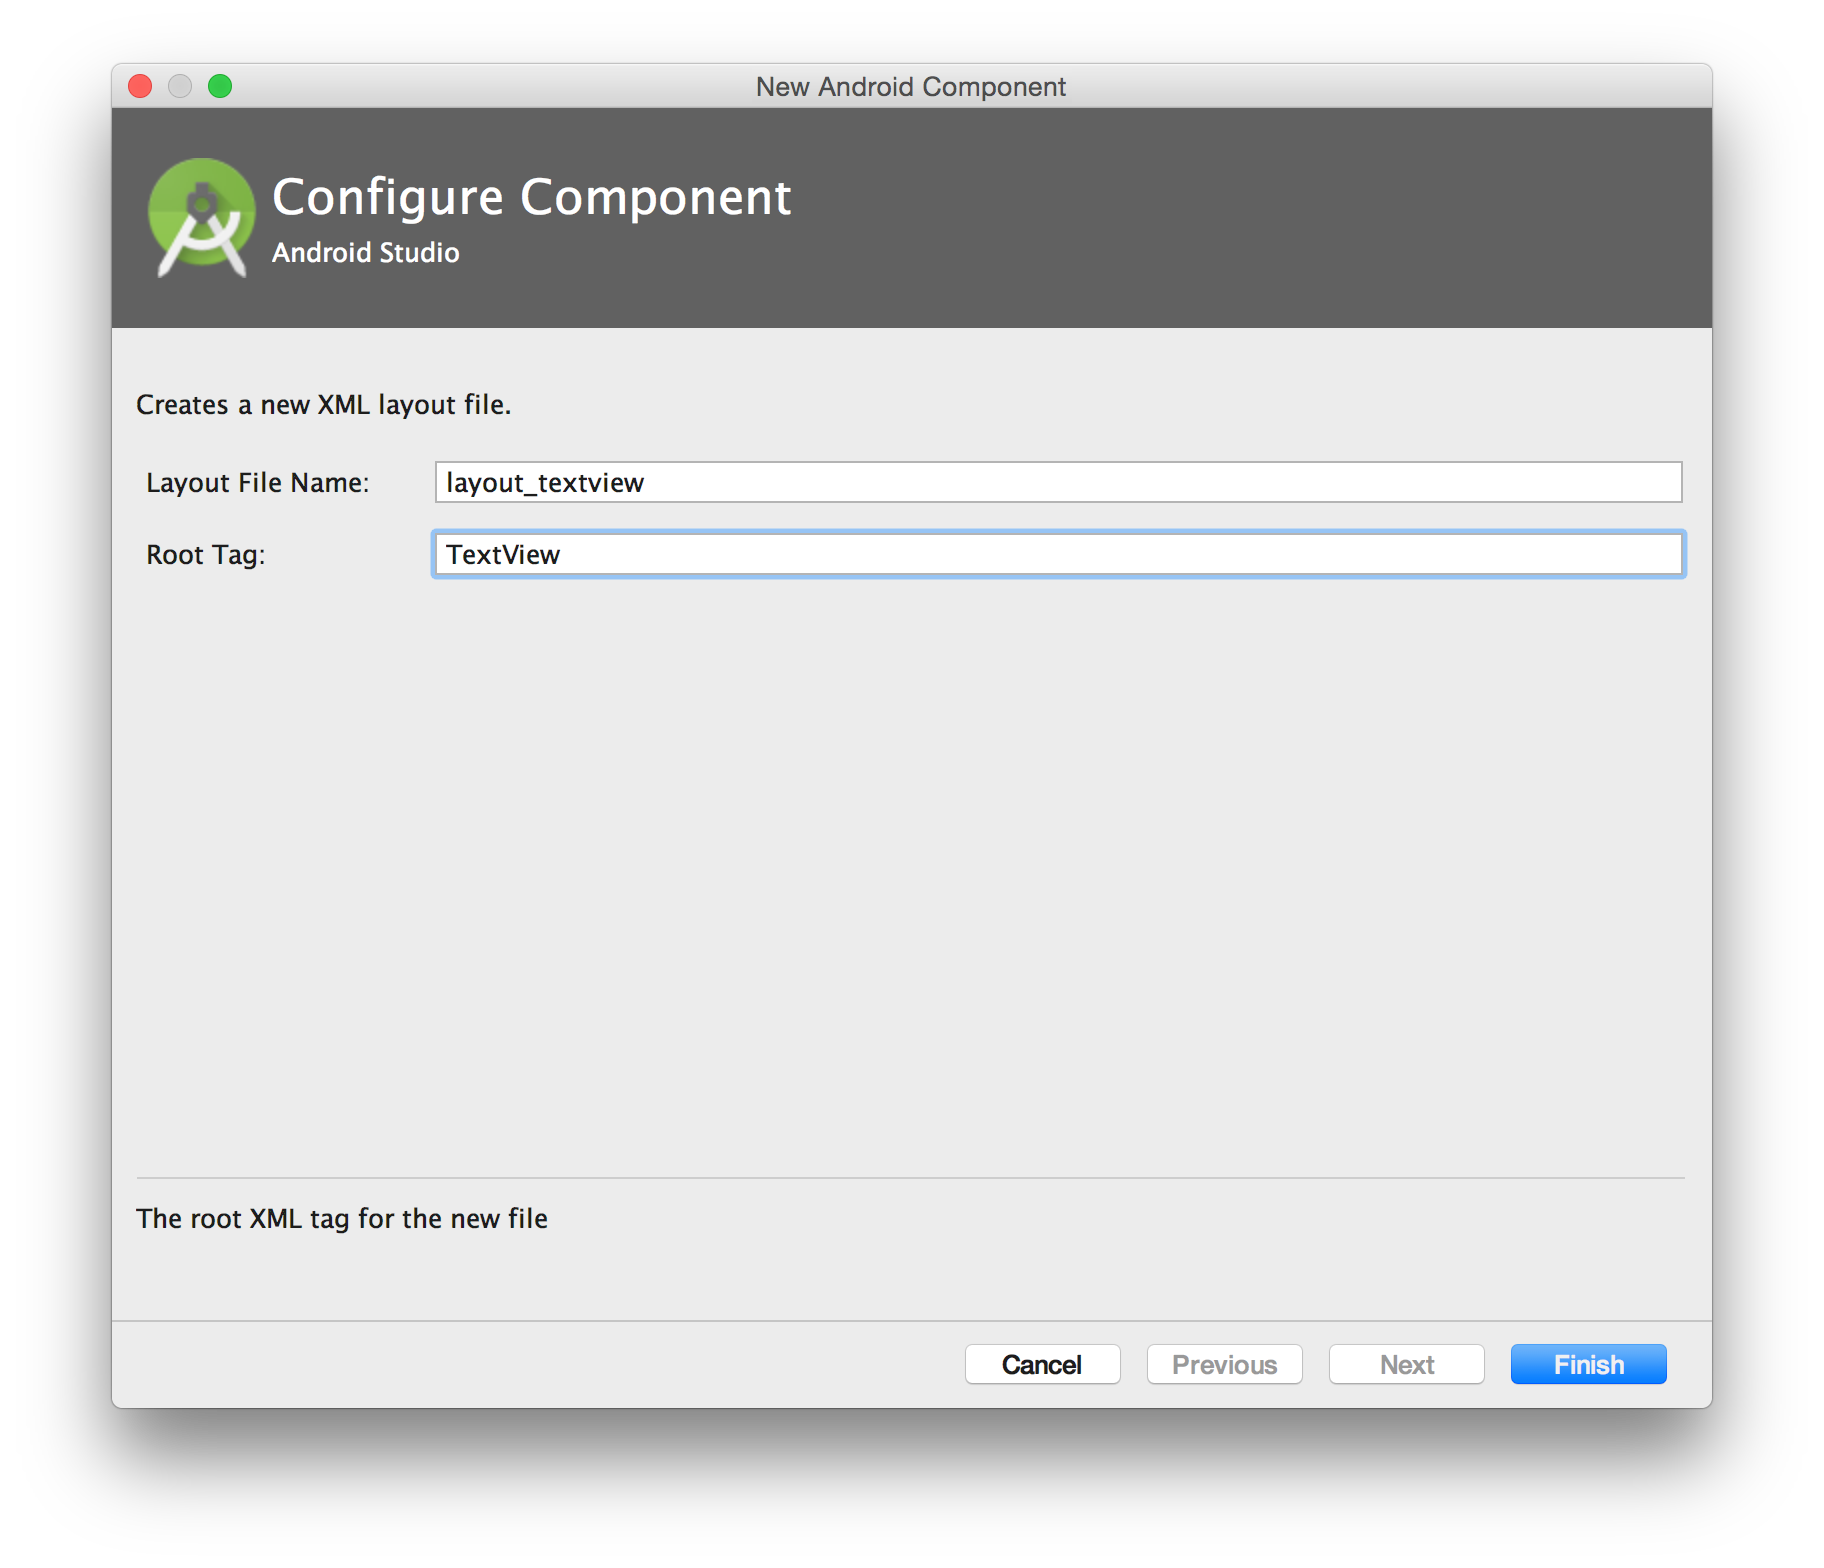
\includegraphics[width=\textwidth]{images/listview_layout_wizard}
\caption{Using the Android Studio wizard to add a new layout XML file}
\label{fig:listview_layout_wizard}
\end{figure}


Now edit layout\_textview as follows:

\begin{lstlisting}
<?xml version="1.0" encoding="utf-8"?>
<TextView xmlns:android="http://schemas.android.com/apk/res/android"
    android:id="@+id/label"
    android:layout_width="fill_parent"
    android:layout_height="fill_parent"
    android:padding="10dp"
    android:textSize="16dp"
    android:textStyle="bold" >
</TextView>
\end{lstlisting}

\paragraph{} This second layout is essentially just the content of each element of the listview that will be displayed. 

\paragraph{} Now finally, we can link all these bits together by editing MainActivity.java. We want to do two things. Firstly, populate the ListView, and secondly, react to clicks on the list by displaying a Toast of the list contents. Our MainActivity.java should look like this:

\begin{lstlisting}
package org.simonwells.listview_example;

import android.support.v7.app.AppCompatActivity;
import android.os.Bundle;
import android.view.View;
import android.widget.AdapterView;
import android.widget.ArrayAdapter;
import android.widget.ListView;
import android.widget.Toast;

public class MainActivity extends AppCompatActivity {

    String[] colourArray = {"Red", "Orange", "Yellow", "Green", "Blue", "Indigo", "Violet"};

    @Override
    protected void onCreate(Bundle savedInstanceState) {
        super.onCreate(savedInstanceState);
        setContentView(R.layout.activity_main);

        ArrayAdapter adapter = new ArrayAdapter<String>(this,
                R.layout.layout_textview, colourArray);
        final ListView listView = (ListView) findViewById(R.id.colour_list);
        listView.setAdapter(adapter);

        listView.setOnItemClickListener(new AdapterView.OnItemClickListener() {
            @Override
            public void onItemClick(AdapterView<?> adapterView, View view, int i, long l) {
                String selection = (String) (listView.getItemAtPosition(i));
                Toast.makeText(getApplicationContext(), selection, Toast.LENGTH_SHORT).show();
            }
        });
    }
}
\end{lstlisting}

\paragraph{} You can now run your app. Assuming that everything has right you should now be able to view a scrollable list of colours of the rainbow (or whatever else you put in the list).

\begin{figure}[H]
\centering
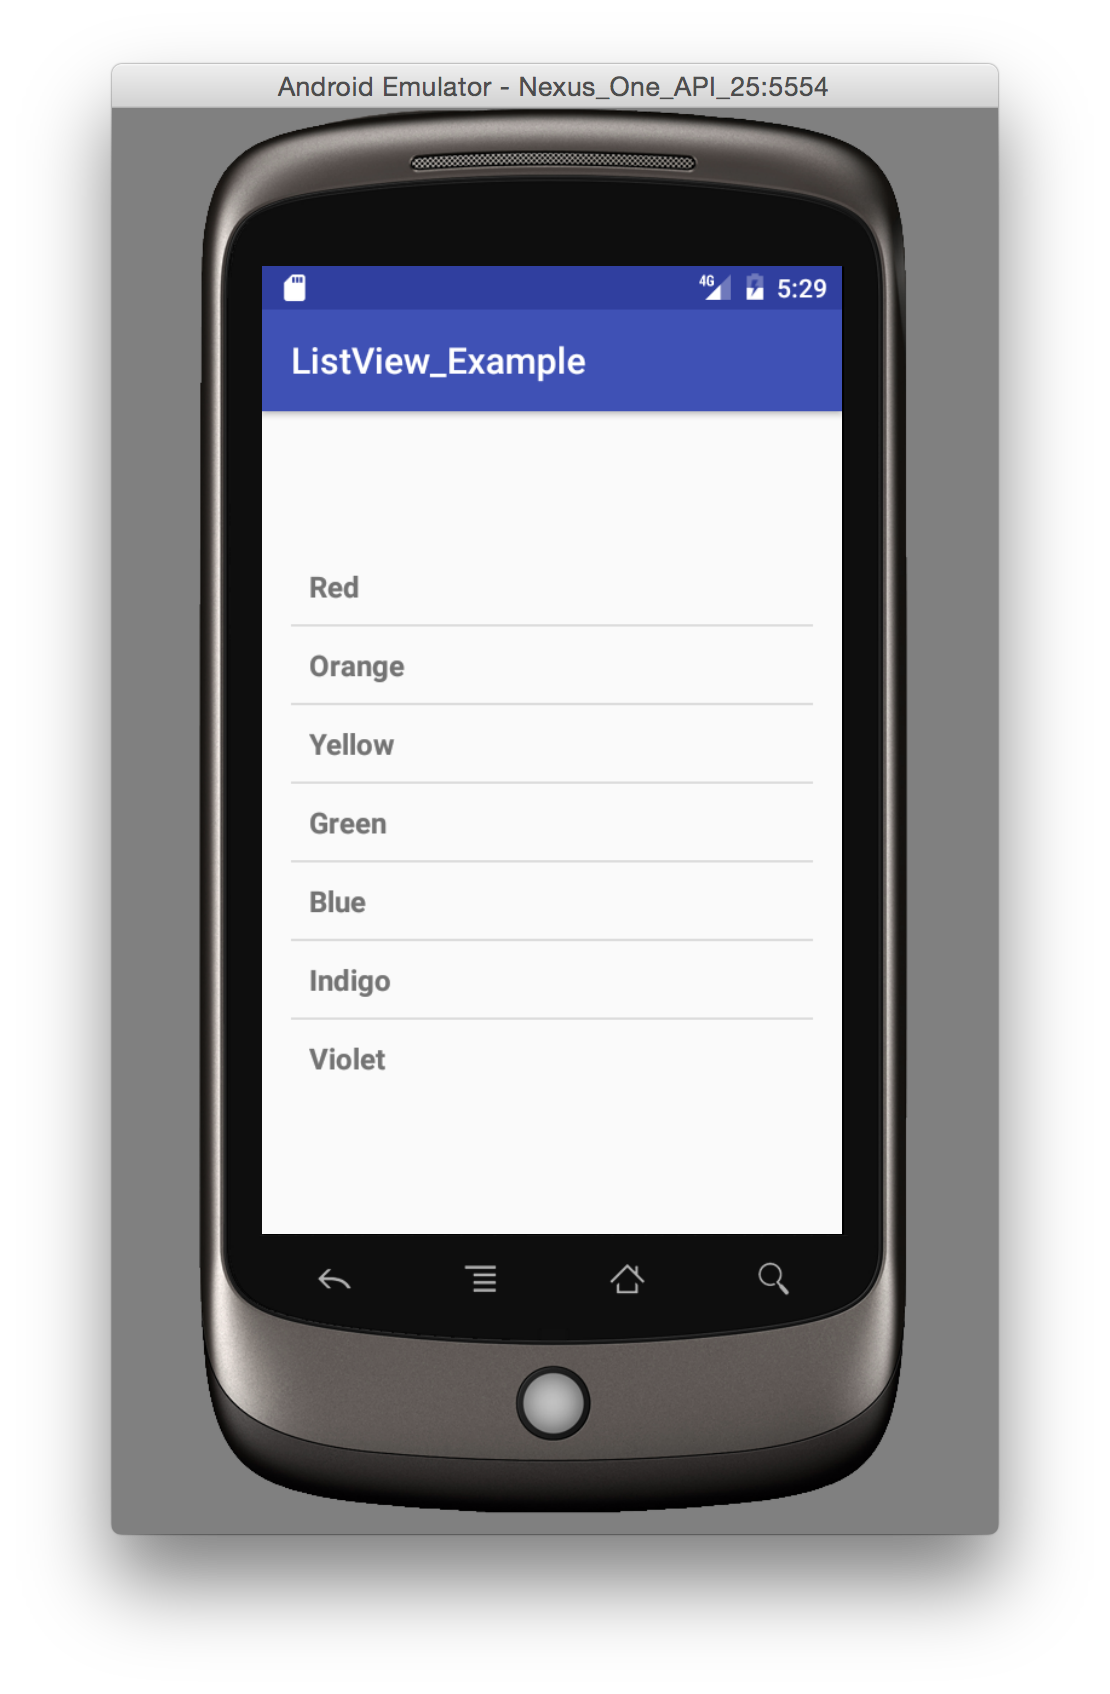
\includegraphics[width=0.8\textwidth]{images/listview_avd}
\caption{AVD showing the listview example app}
\label{fig:listview_avd}
\end{figure}


\paragraph{} We haven't gone into as much detail explaining what is happening in the ListView as in other examples. This is because it is mostly built from things we have already seen. It is a combination of basic views, layouts, and activities glued together with a bit of Java. Once you have it running you should spend some time getting an understanding of how it all fits together.

\paragraph{} In summary, layouts are a powerful and useful way to build flexible and dynamic layouts for your app and are, as a rule, much preferred over hard coding the layouts, especially when dealing with different screen sizes.



%\section{Dialogs (using Fragments)}
%\paragraph{} By default an activity occupies the entire screen. However you can apply a dialog theme so that your activity is displayed as a floating dialog which can sometime be useful to warn users or to double check that a user is sure of their action (when an action could have potentially bad consequences such as deleting data).

\section{Designing Apps}
\paragraph{} You shouldn’t spend months on your app before checking if the design will work. The use of storyboards and navigation maps followed by a rapid development application development tool will help you mock up a template to test your design early on and hopefully find any flaws with your design.

\paragraph{} We will design a home page (default activity displayed when an app is launched by clicking its icon) for an app. You can base this on your coursework idea (if you have one) or any other app that you would like to consider. If you don't have any ideas or want to try something different then perhaps design the home-page for a weather display app:

\begin{framed}
Assume that you have an API available which will allow your device to remotely retrieve information about the weather conditions and perhaps forecast for a named area, e.g. Edinbugh. You can use the data returned by the API of OpenWeathermap\footnote{\url{openweathermap.org}} as an exemplar of what data might be available to you. Design a home page to display this data, or a sensible subset, to your user.
\end{framed}

\begin{itemize}
\item Start will a storyboard for a layout, we will need a home page that will link to a photo gallery of attractions, a page that will link to various tourists sites and a page about our application itself.
\item Decide on a prototyping tool such as PhoneGap\footnote{\url{http://phonegap.com/}}, App Inventor\footnote{\url{http://appinventor.mit.edu/}}, using the XML layout designer in Android Studioor any other tool you feel comfortable using, NB. Try a search for ``Android Wireframe Mockup tools'' and you will be surprised by the number available\footnote{\url{http://mashable.com/2013/04/02/wireframing-tools-mobile/} is a good place to start}. If you are not sure where to start then try the XML Layout Designer of Android Studio as it is already installed in the labs. If you are still unsure there are plenty of comparison articles available online\footnote{\url{http://www.amlcode.com/2010/07/16/comparison-appinventor-rhomobile-phonegap-appcelerator-webview-and-aml/}}.
\item Try and develop the basic layout to the Weather App from above. Alternatively,  spend the time trying to prototype your own coursework app.
\end{itemize}

\section{Summary}
\paragraph{} In this practical we have: 

\begin{itemize}
\item Explored Android Layouts and Views for managing how your UI is displayed.
\item Begun prototyping Android apps using appropriate prototype and mockup tools.
\end{itemize}
